\subsection{A-II Cloud Actors, Management Responsibilities and XMDrive}
\subsubsection{The platform that Company A consumes and the survey service that Company A provides
to respondents}

Company A assumes different roles in different service
relationships: it consumes a cloud provider's platform to deploy
its survey application, while providing the survey service to
respondents.
% ---------- Table: Cloud actors ----------
\begin{table}[H]
\centering
\small

\begin{tabularx}{\textwidth}{
    @{}
    >{\raggedright\arraybackslash}p{0.15\textwidth}
    >{\raggedright\arraybackslash}X
    >{\raggedright\arraybackslash}X
    @{}
}
\toprule

\textbf{Cloud actor}
&
\textbf{Platform service consumed by Company A}
&
\textbf{Survey service provided by Company A}
\\

\midrule

\textbf{Consumer}
&
Company A
&
Survey respondents
\\
\addlinespace

\textbf{Provider}
&
Google Cloud, providing Cloud Run
&
Company A
\\
\addlinespace

\textbf{Carrier}
&
Company A’s ISP (e.g., TM) and other network operators providing connectivity to Google Cloud
&
Respondents’ mobile and fixed-line operators (e.g., Maxis, CelcomDigi)
\\
\addlinespace

\textbf{Broker}
&
None
&
None
\\
\addlinespace

\textbf{Auditor}
&
Google Cloud’s independent SOC 2 Type II auditors (Ernst \& Young LLP or Coalfire, depending on the applicable report)
&
Independent PDPA compliance assessor commissioned by Company A
\\

\bottomrule
\end{tabularx}

\caption{Cloud Actors from Two Service Perspectives}
\label{tab:cloud-actors}
\end{table}
\subsubsection{The division of management responsibility
under IaaS, PaaS and SaaS}

Table~\ref{tab:survey-management} compares
the division of management responsibility under IaaS, PaaS and SaaS.

% ---------- Table: Management responsibilities ----------
\begin{table}[H]
\centering
\small
\begin{tabularx}{\textwidth}{
    @{}
    >{\raggedright\arraybackslash}p{0.24\textwidth}
    *{3}{>{\raggedright\arraybackslash}X}
    @{}
}
\toprule
\textbf{Management responsibility} &
\textbf{IaaS}\newline Self-managed VMs &
\textbf{PaaS}\newline Cloud Run &
\textbf{SaaS}\newline Off-the-shelf survey product \\
\midrule

Hardware and underlying infrastructure &
Provider &
Provider &
Provider \\

Operating system and patching &
Company A (guest OS) &
Provider maintains the host OS. Company A maintains the container image.\textsuperscript{*} &
Provider \\

Application runtime environment &
Company A &
Provider manages the platform. Company A manages the runtime and dependencies.\textsuperscript{*} &
Provider \\

Scaling &
Company A &
Company A sets the maximum instance count. The platform scales automatically. &
Provider \\

Survey application code and maintenance &
Company A &
Company A &
Provider maintains the application. Company A configures its features. \\

Data use, retention and deletion policies &
Company A sets and enforces the policies. &
Company A sets the policies and configures services to enforce them. &
Company A sets the policies and checks whether the product supports them. \\

User roles and application access permissions &
Company A &
Company A &
Company A \\

\bottomrule
\end{tabularx}
\caption{Management responsibilities for Company A's survey service under IaaS, PaaS and SaaS}
\label{tab:survey-management}

\par\smallskip
\begin{minipage}{\textwidth}
\footnotesize
\textsuperscript{*}The Cloud Run option assumes that Company A maintains its own container image.
\end{minipage}
\end{table}

The service model defines what Company A obtains from its provider and
which tasks its IT team manages. The deployment model describes the
cloud environment as public, private, community or hybrid~\parencite{nist2011}.
In the proposed PaaS setup, Company A's three-person team maintains the
survey code and its own container image. Google operates the Cloud Run
platform~\parencite{cloudrun}. If Company A chose IaaS, it could run the same
survey on virtual machines in either a public or a private cloud.
Choosing a service model therefore leaves the deployment model as a
separate decision.

Combining SaaS, PaaS and IaaS within one public cloud does not create
a hybrid cloud. A hybrid cloud requires distinct cloud environments
connected in a way that lets data and applications move between
them~\parencite{nist2011}. Similarly, a Google Cloud VPC gives Company A a
virtual network isolated from other VPC networks~\parencite{googlevpc}.
The deployment remains public because the cloud infrastructure is
offered for use by the general public~\parencite{nist2011}. A private cloud
requires infrastructure reserved for one organisation's exclusive
use~\parencite{nist2011}, so creating a VPC within a public cloud does not,
by itself, establish a private cloud.



\subsubsection{XMDrive Analysis}
\paragraph{Service Model}

XMDrive is \textbf{SaaS}. The provider manages the application, runtime,
operating system, and underlying infrastructure. Students manage their
own files and sharing settings.

Students have limited configuration options. For example, in Basic
Settings, they can choose the language, the number of items per page,
and the default sort order, as shown in
Figure~\ref{fig:xmdrive-basic-settings}.. Students cannot change their storage quota
themselves.

\begin{figure}[H]
    \centering
    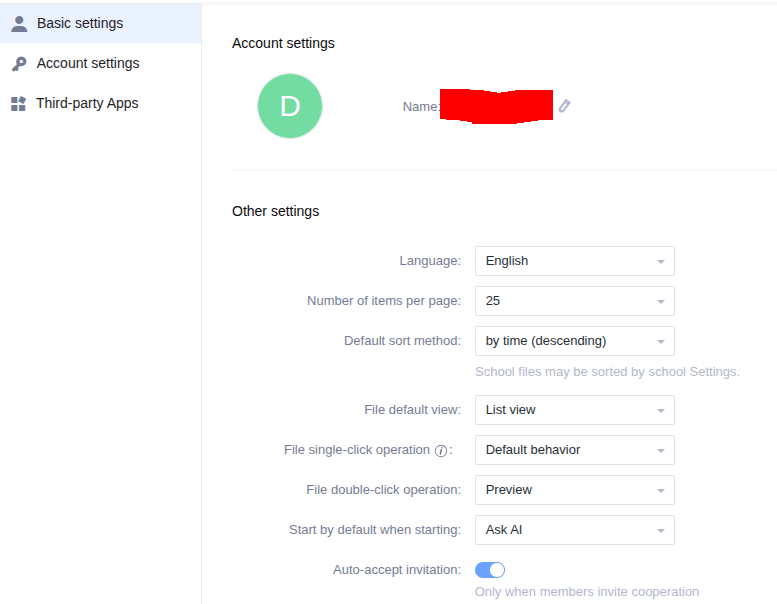
\includegraphics[width=1\linewidth]{images/part-a-2/xmdrive-basic-settinggs.png}
    \caption{XMDrive Basic Settings}
    \label{fig:xmdrive-basic-settings}
\end{figure}

\paragraph{Deployment Model}
The official documentation does not provide detailed information regarding the fact that XMDrive's underlying cloud infrastructure is provisioned exclusively for XMUM. But IPinfo lists XMUM in the
\textit{Company} field for the IP address \texttt{218.208.8.50}, as shown in
Figure\ref{fig:xmdrive-ipinfo}.
\begin{figure}[H]
    \centering
    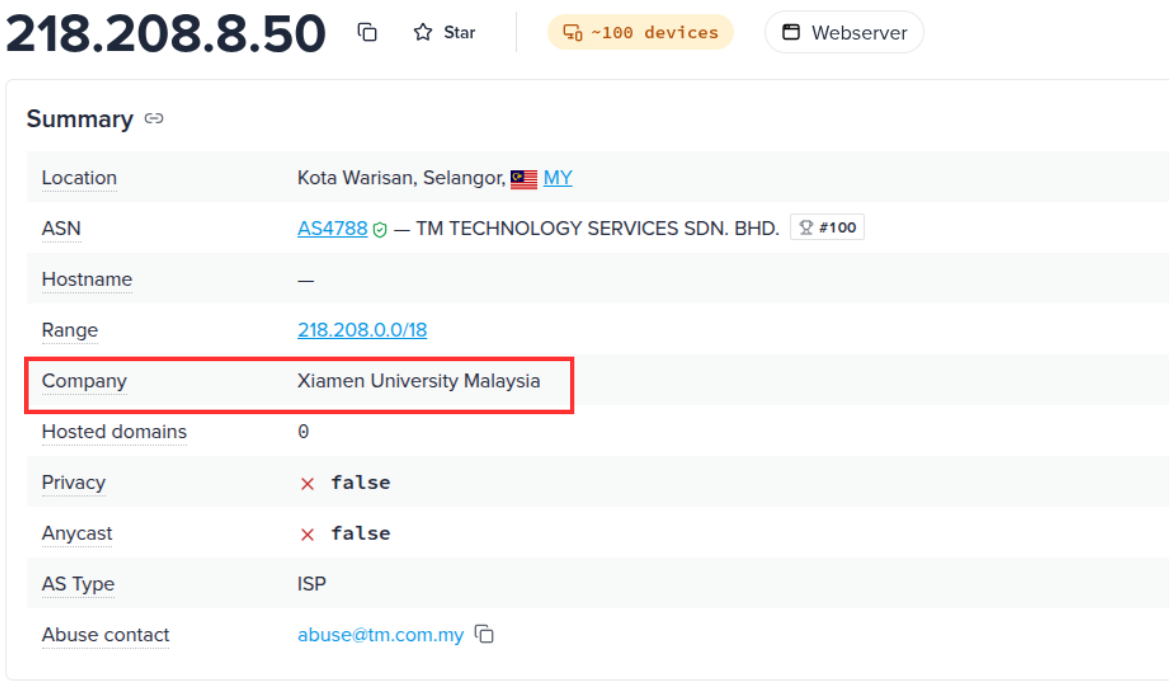
\includegraphics[width=1\linewidth]{images/part-a-2/xmdrive-ipinfo.png}
    \caption{XMDrive Ipinfo}
    \label{fig:xmdrive-ipinfo}
\end{figure}


Under this assumption, XMDrive is classified as a \textbf{private cloud}. Because
its cloud infrastructure
provisioned for the exclusive use of XMUM.

\paragraph{NIST characteristics it shows clearly or partly}
\begin{table}[H]
\centering
\caption{NIST Cloud Characteristics in XMDrive}
\label{tab:xmdrive-nist}
\begin{tabularx}{\linewidth}{@{}p{0.23\linewidth}lX@{}}
\hline
\textbf{Characteristic} & \textbf{Extent} & \textbf{Evidence} \\
\hline

Broad network access & Clearly &
The university website states that students can access XMDrive on and
off campus using different devices and web browsers~\parencite{xmum-online-storage}. \\

On-demand self-service & Partly &
Students can upload files to \textit{Personal files} on their own.
They cannot increase or decrease their storage quota themselves. \\

Resource pooling & Partly &
XMDrive provides separate storage spaces for individuals and
organisational units within the same service. Whether the underlying
storage is dynamically allocated from a shared resource pool remains
unconfirmed. \\

Rapid elasticity & Partly &
The personal storage quota is 5.00~GB, and students cannot increase
it themselves. Changes in student enrolment from year to year may
affect overall storage demand. Whether the underlying storage capacity
can scale rapidly with demand remains unconfirmed. \\

Measured service & Clearly &
The \textit{Personal files} panel displays
\texttt{Used: 0 B / 5.00 GB}, as shown in
Figure~\ref{fig:xmdrive-personal-storage}. \\

\hline
\end{tabularx}
\end{table}
\begin{figure}[H]
    \centering
    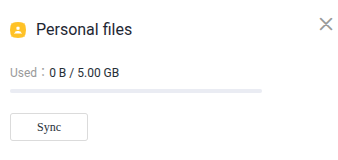
\includegraphics[width=1\linewidth]{images/part-a-2/personalstorage.png}
    \caption{XMDrive Personal Storage}
    \label{fig:xmdrive-personal-storage}
\end{figure}
